%%=============================================================================
%% Resultaten
%%=============================================================================

\chapter{Resultaten}
\label{ch:resultaten}

\section{Stappenplannen testgevallen}

\subsection{Terugkerende stappen}
\label{recurringsteps}

Hier worden stappen gedefiniëerd die doorheen de testgevallen gebruikt worden.

\begin{enumerate}
    \item 
    \label{factoryreset}
    Het apparaat moet worden teruggezet naar de fabrieksinstellingen, en alle data moet worden gewist. Dit kan gedaan worden door binnen de instellingen applicatie te navigeren naar 'Systeem' > 'Opties voor resetten' > 'Alle gegevens wissen (fabrieksinstellingen terugzetten)'. Hier moet 'interne opslag wissen' aangeduid worden, voordat er op 'telefoon resetten' wordt gedrukt, zoals te zien in figuur \ref{fig:fabrieksinstellingen}. Bevestig deze actie door de pincode van het apparaat in te vullen, indien deze is ingesteld. Druk hierna op 'Alles wissen'. De telefoon wordt nu gereset en heropgestart.
    \item 
    \label{initialsetup}
    Wanneer de telefoon teruggezet is naar de fabrieksinstellingen, zal er gevraagd worden om de initïele setup opnieuw te voltooien. Hier moet telkens de standaard optie aangeduid worden, behalve als er hier wordt vermeld een andere optie te nemen.
    \begin{itemize}
        \item Apps en gegevens kopiëren: druk op 'gegevens niet kopiëren'. We willen hier met een 'vers' Android besturingssysteem werken.
        \item Inloggen met Google: Kies hier om een nieuw account aan te maken.
        \item Gezichtsontgrendeling: Dit heeft geen belang voor dit experiment, en mag overgeslaan worden.
        \item Vingerafdruk ontgrendeling: Dit heeft geen belang voor dit experiment, en mag overgeslaan worden.
        \item Google Pay: Dit heeft geen belang voor dit experiment, en mag overgeslaan worden.
    \end{itemize}
    \item 
    \label{setupgoogleapps}
    Stel de Google applicaties in. Ga één voor één door de applicaties in figuur \ref{fig:googleapps} en doorloop  het initële setup proces. Wanneer er gevraagd wordt om machtigingen te verlenen aan de applicatie, druk dan op toestaan.
\end{enumerate}

\begin{figure}
    \centering
    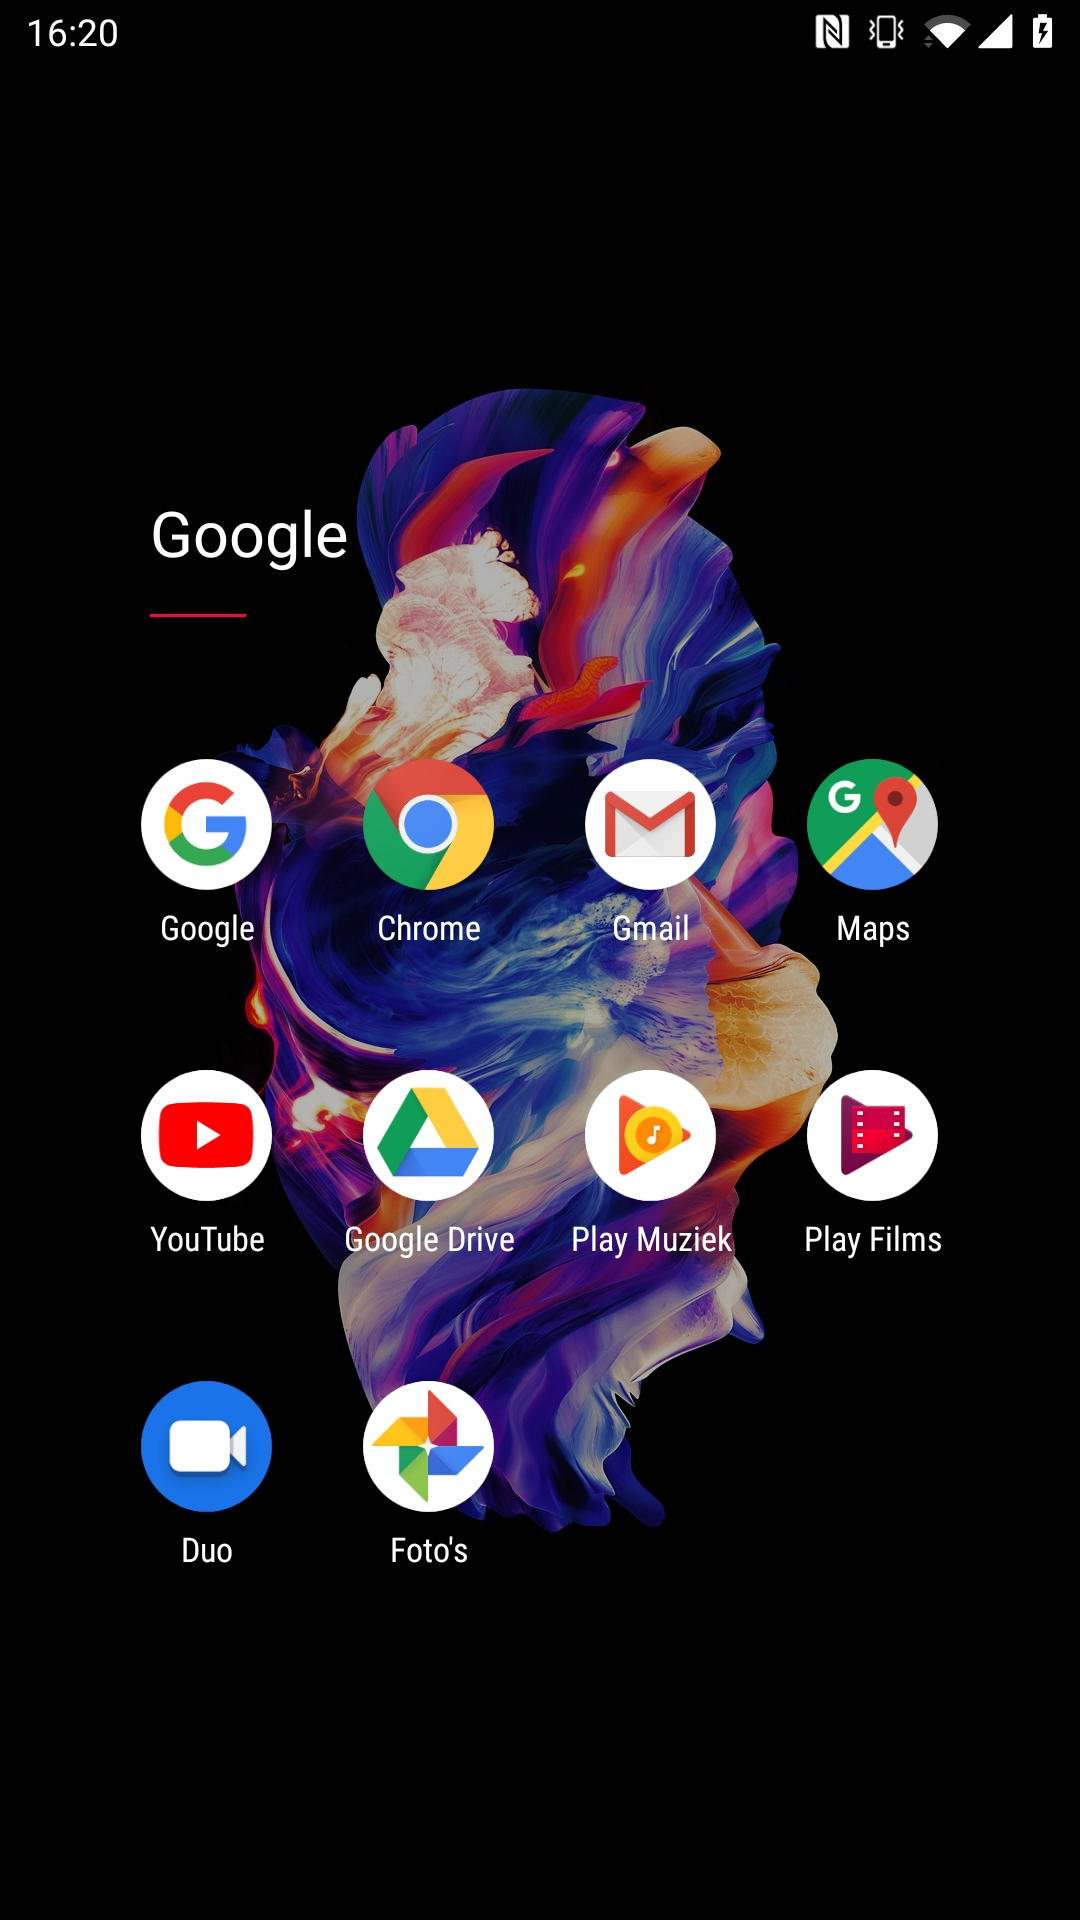
\includegraphics[width=0.4\textwidth]{img/googleapps.jpg}
    \caption{Screenshot van de google applicaties die moeten worden geopend en ingesteld}
    \label{fig:googleapps}
\end{figure}

\subsection{Testgeval 1: Android met fabrieksinstellingen}

Voor de toestand van dit testgeval te bekomen, moeten volgende stappen uitgevoerd worden.
\begin{enumerate}
    \item Stap \ref{factoryreset} van terukerende stappen (\ref{recurringsteps})
    \item Stap \ref{initialsetup} van terukerende stappen (\ref{recurringsteps})
    \item Stap \ref{setupgoogleapps} van terukerende stappen (\ref{recurringsteps})
\end{enumerate}


\subsection{Testgeval 2: Android met aangepaste instellingen}

Voor de toestand van dit testgeval te bekomen, moeten volgende stappen uitgevoerd worden.

\begin{enumerate}
    \item Stap \ref{factoryreset} van terukerende stappen (\ref{recurringsteps})
    \item Stap \ref{initialsetup} van terukerende stappen (\ref{recurringsteps})
    \item Stap \ref{setupgoogleapps} van terukerende stappen (\ref{recurringsteps})
\end{enumerate}
    

\subsection{Testgeval 3: Aangepaste versie van Android}

\section{Monitoring netwerkactiviteit}

\subsection{Testgeval 1: Android met fabrieksinstellingen}

\subsection{Testgeval 2: Android met aangepaste instellingen}

\subsection{Testgeval 3: Aangepaste versie van Android}